\documentclass{ieeetj}

\usepackage{cite}
\usepackage{amsmath,amssymb,amsfonts}
\usepackage{graphicx,color}
\usepackage{textcomp}
\usepackage{xcolor}
\usepackage{hyperref}
\hypersetup{hidelinks=true}
\usepackage{booktabs}
\usepackage{multirow}
\let\labelindent\relax
\usepackage{enumitem}
\usepackage{tikz}
\usetikzlibrary{positioning,arrows.meta,fit}

% IEEE OJCS Specific Color Definitions
\AtBeginDocument{\definecolor{tmlcncolor}{cmyk}{0.93,0.59,0.15,0.02}\definecolor{NavyBlue}{RGB}{0,86,125}}

% Logo Placeholders (Required by ieeetj)
\def\OJlogo{\vspace{-4pt}$<$Society logo(s) and publication title will appear here.$>$}
\def\seclogo{\vspace{10pt}$<$Society logo(s) and publication title will appear here.$>$}

\def\authorrefmark#1{\ensuremath{^{\textbf{#1}}}}
\newcommand{\todo}[1]{\textcolor{red}{[#1]}}

\begin{document}

\receiveddate{XX Month, XXXX}
\reviseddate{XX Month, XXXX}
\accepteddate{XX Month, XXXX}
\publisheddate{XX Month, XXXX}
\currentdate{13 October, 2026}
\doiinfo{XXXX.2026.1234567}

\title{Balancing Security and Usability: Adaptive CAPTCHA Orchestration via Reinforcement Learning}

\author{Anonymous Author(s)}
\affil{Affiliation Omitted for Double-Anonymized Review}

\begin{abstract}
Websites increasingly receive a continuous bot-likelihood score for each user instead of a pass/fail decision, but turning that score into an action (no challenge, a CAPTCHA of some difficulty, or a block) is still left to hand-written rules. We study whether reinforcement learning (RL) can learn this mapping over an 11-level action ladder. A small LSTM \emph{Humanity Scorer} reads mouse dynamics (displacement, inter-event time, speed and acceleration); its calibrated output, a running session score, challenge history and the number of active users form the state of a DQN, PPO, Neural-LinUCB or Neural Thompson Sampling controller. All evaluation is simulated: bots solve challenges stochastically (an item-response model), and human pass rates, solve times and abandonment are taken from published CAPTCHA user studies, so usability is \emph{modelled, not measured}. On a held-out block of recordings never used for scorer or policy training, DQN reaches a Discrimination Index (humans kept \% $-$ bots through \%) of 98.9 (95\% CI $\pm$0.4 over 5 training seeds) against 78.7 for the best static threshold policy; removing the Humanity Score drops it to 23.6. When challenges are solved stochastically, Thompson Sampling matches or exceeds DQN (91.5 vs 88.6). We also report the limits of the approach: rewards computed only from observable challenge outcomes collapse to ``never challenge'', and when the scorer is miscalibrated (covert bots or bot-like humans), frozen RL policies degrade faster than static thresholds, while online training recovers only when its reward does not inherit the scorer's error.
\end{abstract}

\begin{IEEEkeywords}
Behavioural biometrics, bot detection, CAPTCHA, calibration, contextual bandits, mouse dynamics, reinforcement learning, web security.
\end{IEEEkeywords}

\maketitle

\section{INTRODUCTION}
\IEEEPARstart{A}{utomated} traffic is now close to half of all web requests, and 37\% of 2024 traffic was attributed to malicious bots \cite{imperva2025}. Bots scrape content \cite{mazilu2022}, post spam \cite{ferrara2016} and stuff credentials \cite{ba2021}. The standard defence is the CAPTCHA \cite{von_2003,guerar2021}, but every challenge also costs legitimate users time and some of them leave: in a large field study, humans solved distorted-text CAPTCHAs correctly only 71--98\% of the time depending on the scheme \cite{bursztein_humans_2010}, and in a recent study of modern CAPTCHAs a substantial share of participants abandoned the task when a challenge was presented \cite{captcha_study_2023}. At the same time, vision-language models now solve many visual challenges \cite{qi2026,wu2025mca_bench}, and reCAPTCHA v2 has been broken with off-the-shelf detectors \cite{plesner2024yolo}.

Risk-based services such as reCAPTCHA v3 therefore return a continuous score rather than a decision \cite{reCAPTCHA}. That moves the hard part to the website operator, who must decide what to do with a score of, say, 0.6. Three things make this decision hard in practice. \emph{(i) One threshold does not fit every context}: a score that justifies frictionless browsing may be inadequate for a payment page \cite{sepczuk_2018}, and fixed thresholds become stale as adversaries adapt \cite{sethi_2018,sivakorn_recaptcha_2016}. \emph{(ii) Scores are not comparable across providers}: each detector has its own undisclosed calibration, so combining them is ad hoc \cite{yousef_2023}. \emph{(iii) The trade-off is sequential}: a mild first challenge can be escalated if the user still looks suspicious, and a policy that challenges early can relax later. Rule-based web application firewalls \cite{cloudArmour} encode these choices by hand.

This paper asks whether an RL controller can learn the score-to-action mapping, and what can and cannot be concluded from a simulation-based evaluation of it. Our contributions are:
\begin{enumerate}[label=\roman*), leftmargin=*, itemsep=1pt]
\item \textbf{A graduated orchestration formulation.} The controller chooses one of 11 levels (0: no challenge; 1--9: increasingly strong challenges; 10: block) every 10\,s of a session, using a behavioural score and session and server context (Section~\ref{sec:method}).
\item \textbf{A compact, calibrated behavioural scorer} (6{,}081 parameters, temperature-scaled), chosen by grouped cross-validation, together with the data protocol needed to avoid leakage between scorer, policy and evaluation (Section~\ref{sec:data}).
\item \textbf{A literature-grounded simulator} in which bots solve challenges with a probability that depends on their capability, and human pass rates, solve times and abandonment rates come from published user studies \cite{bursztein_humans_2010,captcha_study_2023} (Section~\ref{sec:env}).
\item \textbf{An evaluation with confidence intervals} of DQN, PPO, Neural-LinUCB and Neural Thompson Sampling against static threshold policies and an ablation without the score, on held-out recordings over 5 training seeds (Section~\ref{sec:results}).
\item \textbf{Negative results that bound deployment}: label-free rewards, and the behaviour of offline and online-trained policies when the scorer's calibration drifts (Sections~\ref{sec:deploy}--\ref{sec:drift}).
\end{enumerate}

\textbf{Scope.} Table~\ref{tab:scope} separates what was evaluated from what is only proposed. In particular, no real CAPTCHA provider, user study, server-load model or adaptive attacker is part of the evaluation; we therefore make no claim about denial-of-service mitigation in the sense of server resources, only about robustness to the volume and composition of bot traffic.

\begin{table}[!t]
\caption{Scope of the Evaluation}
\label{tab:scope}
\centering
\footnotesize
\setlength{\tabcolsep}{3pt}
\begin{tabular}{p{0.30\columnwidth}p{0.62\columnwidth}}
\toprule
\textbf{Status} & \textbf{Component} \\
\midrule
Evaluated & LSTM scorer on our recordings; RL and static policies in simulation; 11 abstract levels with literature-based human/bot outcome models; bot volumes 20--1000; scorer-calibration drift with external data \\
Implemented, not evaluated & Playground website and telemetry collection; web SDK \\
Proposed only & Mobile SDKs, device fingerprinting, routing to real CAPTCHA providers, server-load (DoS) features, adaptive/VLM attackers, user study \\
\bottomrule
\end{tabular}
\end{table}

\section{RELATED WORK}
\textbf{CAPTCHA security and usability.} CAPTCHAs were introduced as hard AI problems \cite{von_2003} and have been surveyed extensively \cite{guerar2021,umar_2022}. Their usability cost is well documented: Yan and El~Ahmad analysed design factors \cite{yan2008captcha}, Bursztein et al.\ measured human accuracy and solve times on 318{,}000 CAPTCHAs from 21 schemes \cite{bursztein_humans_2010}, and Searles et al.\ measured solve times, preferences and abandonment for modern challenges with 1{,}400 participants \cite{captcha_study_2023}. On the attack side, text CAPTCHAs have generic solvers \cite{bursztein2014new}, reCAPTCHA has been bypassed with audio and image models \cite{sivakorn_recaptcha_2016,plesner2024yolo}, its v3 score has been gamed with RL \cite{akrout2019}, and multimodal models solve visual-reasoning challenges \cite{qi2026,wu2025mca_bench,clip_2021}.

\textbf{Behavioural biometrics.} Mouse dynamics separate humans from bots and individuals from each other \cite{khan_2023,shen_2013,antal_2019}. Human motion follows Fitts' law with motor noise \cite{fittslaw2019}, while bots range from straight-line movers to B\'ezier-curve and learned trajectory generators \cite{bezier2025,bezier_bots_2022,antal_2021_sapi}. Iliou et al.\ combined web logs and mouse biometrics to detect advanced web bots \cite{iliou_2021}; Acien et al.\ did so with touch and sensor data \cite{acien_2021}. Recurrent networks are a common choice for such sequences \cite{hochreiter_lstm_1997,wei2021deeplearning}.

\textbf{Adaptive challenges and RL.} Aura-CAPTCHA uses RL and GANs to adapt challenge difficulty \cite{aura_captcha_2025}; it does not orchestrate a graded ladder ending in a block. Contextual bandits choose an action from features to maximise immediate reward \cite{li_linucb_2010,russo_ts_2018}; DQN \cite{mnih_dqn_2015} and PPO \cite{schulman_ppo_2017} optimise discounted return in a Markov decision process \cite{sutton2018reinforcement}, and RL has been applied to fraud detection \cite{cui_2025} and anomaly detection \cite{huang_2018}. Publicly available labelled human/bot interaction data remain scarce \cite{mvula_2023}, which is why we report data sizes and leakage controls in detail.

\section{METHODOLOGY}
\label{sec:method}

\subsection{System Architecture}
Fig.~\ref{fig:system_architecture} shows the four tiers. \emph{Tier 1} (client telemetry) collects cursor coordinates and timestamps in the browser and normalises them to a platform-independent JSON format; only the web version exists. \emph{Tier 2} (Humanity Scorer) converts each 10-second chunk of telemetry into a bot probability; any scorer with a probabilistic output, including a commercial one, can be substituted. \emph{Tier 3} (RL controller) maps the score and context to a level. \emph{Tier 4} (fulfilment) would route each level to a concrete challenge; in this paper levels are simulated (Section~\ref{sec:env}), not served by real providers.

\begin{figure}[!t]
  \centering
  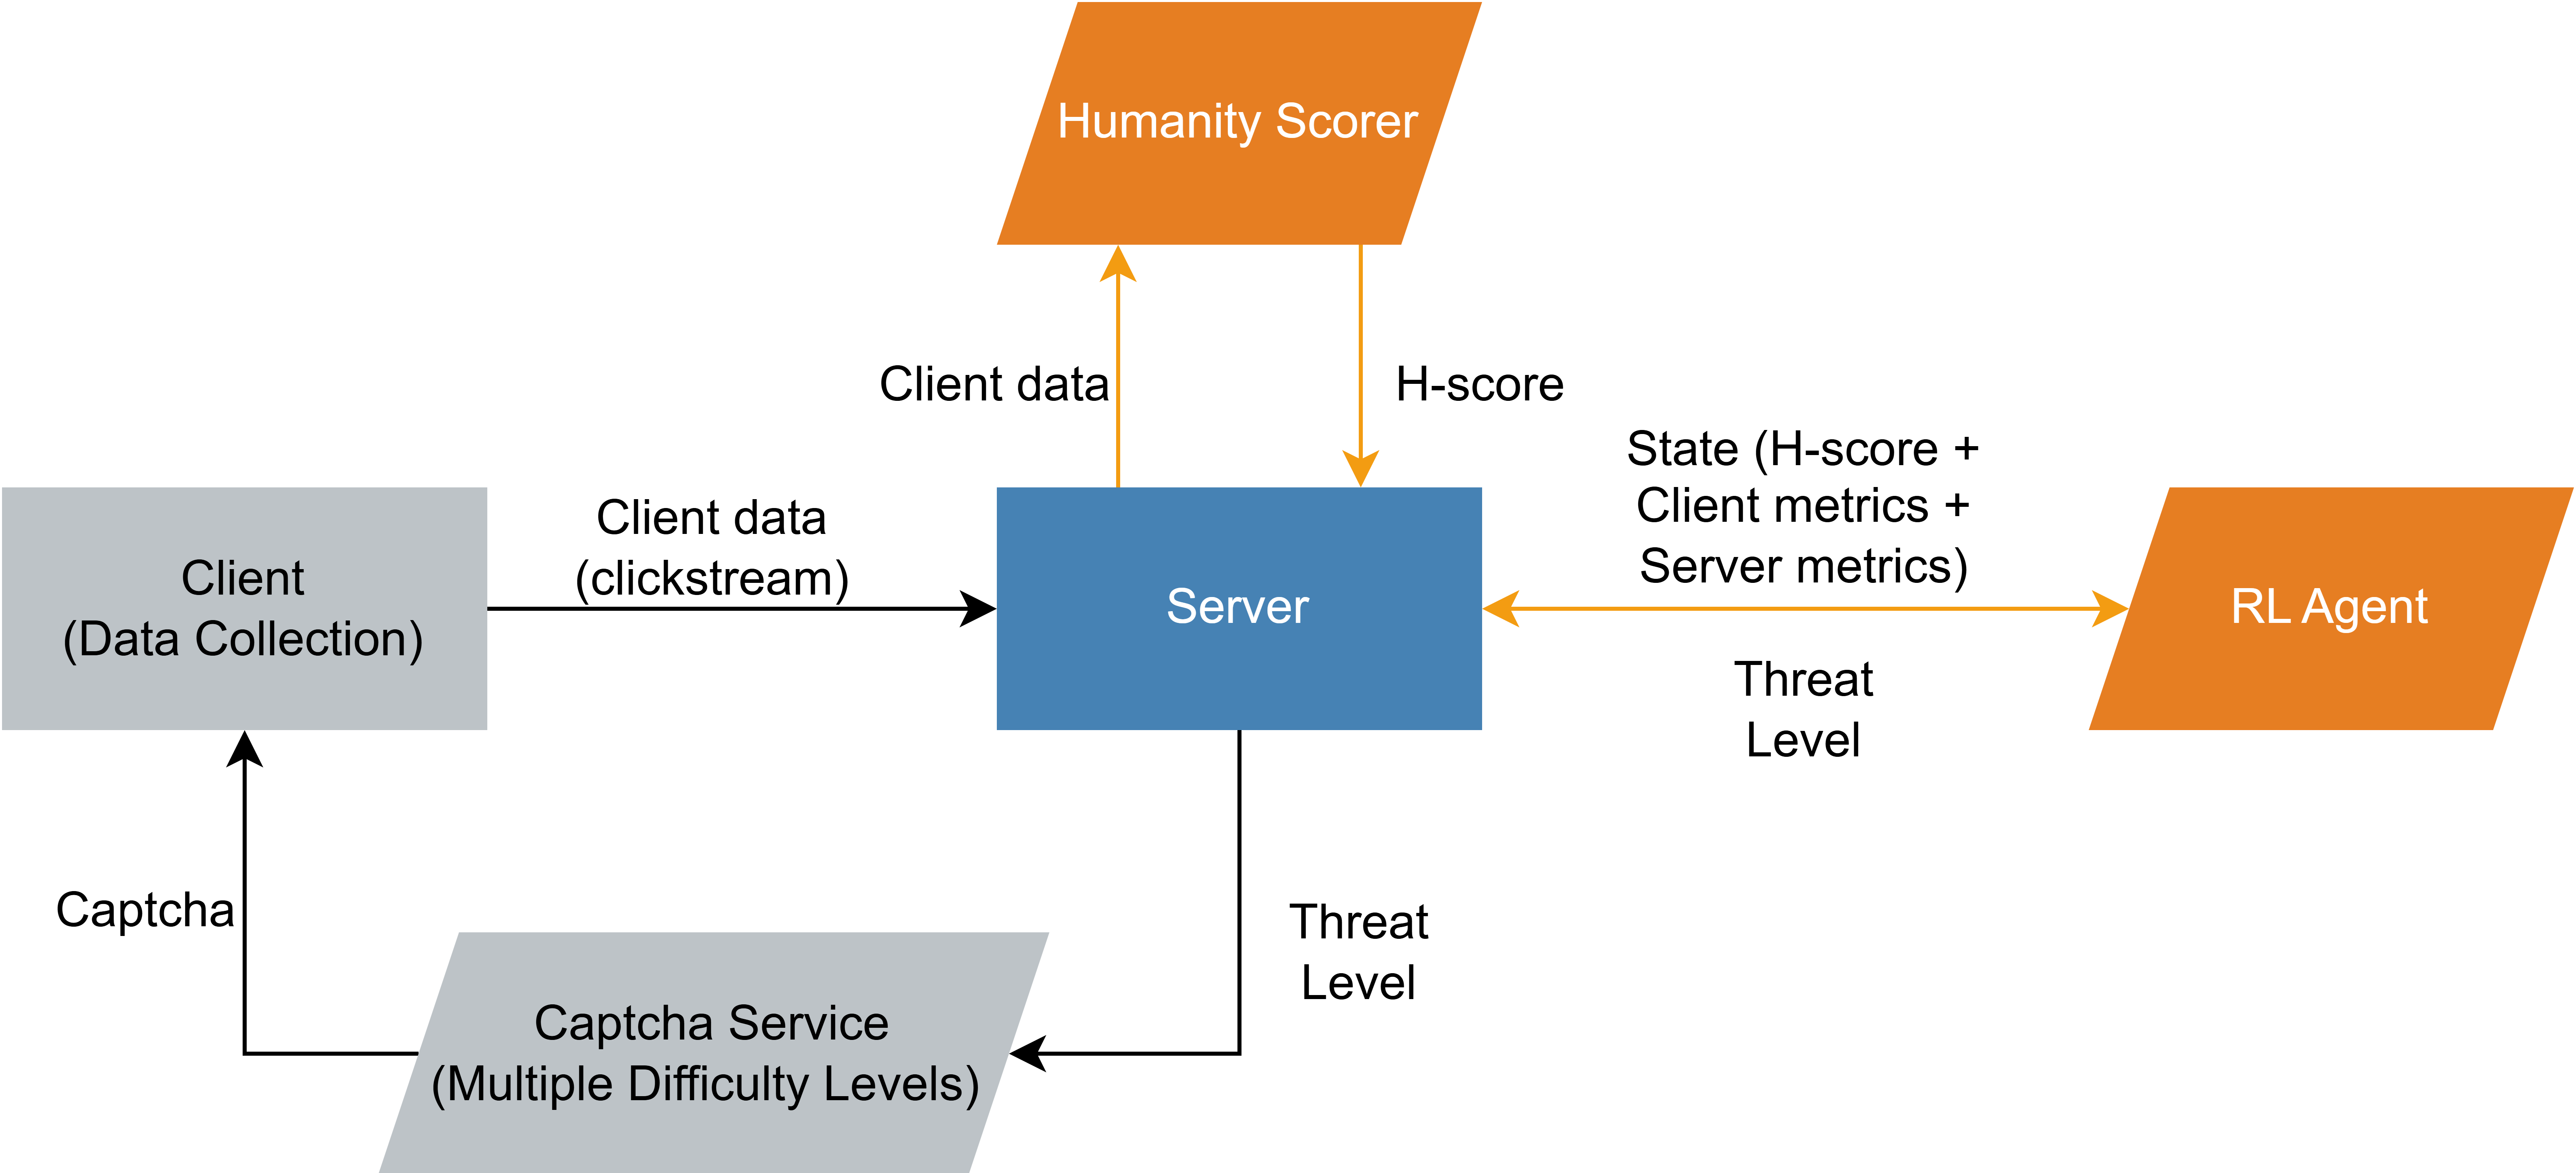
\includegraphics[width=0.95\columnwidth]{images/system_architecture.png}
  \caption{Modular architecture. Tiers 1--3 are implemented; tier 4 is simulated in this paper (Table~\ref{tab:scope}).}
  \label{fig:system_architecture}
\end{figure}

\subsection{Data Collection}
\label{sec:data}
A playground blog website (navigation, form filling, commenting) recorded \texttt{mousemove} events $(x, y, t)$ with a minimum gap of 10\,ms. Each session lasted about 120\,s. Four bot generators of increasing sophistication interacted with the same site: \emph{naive} bots that jump directly to targets, \emph{human-like} bots that move in straight lines at constant speed, \emph{mimic} bots that follow B\'ezier curves with varying speed \cite{antal_2021_sapi}, and \emph{fallible} bots that add overshoots, hesitations and corrections. In total we have \textbf{156 recordings}: 44 human and 112 bot recordings, 42{,}913 movements, from two collection campaigns three months apart. The 44 human recordings come from \textbf{3 participants}.

\textbf{Ethics.} The study followed established ethical guidelines for research with human participants. Participants gave informed consent, and only anonymous cursor trajectories were stored; no personally identifiable information was retained.

\textbf{Partition (answers R1.2).} The split is made \emph{at the recording level, before any windowing or augmentation}, so no window of a recording appears in two blocks. Recordings are divided into a scorer block, an RL block and a held-out \emph{evaluation block} using rotating folds; the results in this paper use fold~2, whose evaluation block has 14 human and 36 bot recordings and is never used to fit or select the scorer or the policy. Within the scorer block we cross-fit five scorers so that every RL training session is scored by a model that did not see it. Every opening of the evaluation block is logged. No augmentation is used (Section~\ref{sec:scorer}). With three participants, the human data cannot support claims about the general population; we report a leave-one-campaign-out check as the closest proxy for unseen users.

\subsection{Humanity Scorer}
\label{sec:scorer}
\textbf{Input.} A chunk (the movements in one 10\,s step) is converted to per-event features $[\Delta x, \Delta y, \Delta t, v, a]$: displacement, inter-event time, speed $v=\lVert(\Delta x,\Delta y)\rVert/\Delta t$ and its first difference $a$. Absolute screen position is deliberately not used, because it encodes page layout rather than behaviour. Features are standardised with training-set statistics and cut into windows of 32 events; the last window is padded and a sixth binary channel marks padded steps (Fig.~\ref{fig:lstm}).

\textbf{Model.} One LSTM layer \cite{hochreiter_lstm_1997} with 32 units reads the window; its final hidden state passes through a 32-unit ReLU layer and a sigmoid output (6{,}081 parameters). Window probabilities are temperature-scaled \cite{guo_calibration_2017} ($T=1.45$) and averaged over the chunk, giving $q = P(\text{bot})$; the Humanity Score is $H = 1-q$. Training uses binary cross-entropy, Adam (learning rate $3\times10^{-3}$), dropout 0.25, recurrent dropout 0.2 and early stopping on validation loss.

\textbf{Why this design.} The original submission used two LSTM layers (200 and 100 units, 304{,}049 parameters) on absolute $(x,y)$ coordinates. A grouped 5-fold search over architectures and input representations on all 156 recordings showed that the original model had about 1{,}170 parameters per training window, that a single 32-unit layer on relative motion was better on every criterion (cross-validated session AUC 0.977 vs 0.906; leave-one-campaign-out AUC 0.890 vs 0.842), and that Gaussian or jitter augmentation did not help a correctly sized model. Adding timing on top of displacement changed AUC by $+0.007$ on average, with inconsistent sign, so we make no claim that timing features are essential; we keep them because acceleration-type features are standard in mouse-dynamics work \cite{khan_2023}.

\begin{figure}[!t]
\centering
\resizebox{\columnwidth}{!}{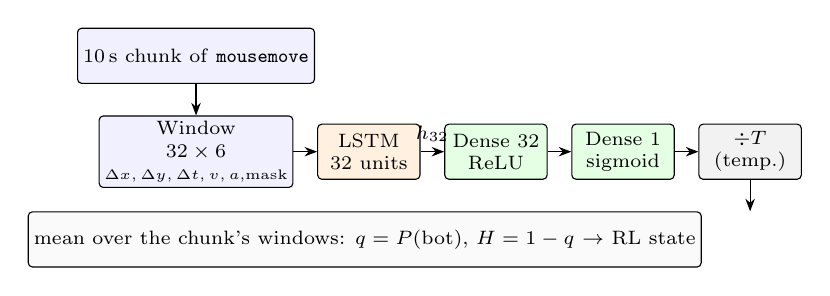
\begin{tikzpicture}[
  font=\scriptsize, node distance=3.0mm,
  box/.style={draw, rounded corners=1.5pt, align=center, minimum height=7mm, inner sep=2pt, fill=#1},
  box/.default=white, >={Stealth[length=1.6mm]}]
\node[box=blue!6, minimum width=16mm] (in) {Window\\$32\times6$\\{\tiny $\Delta x,\Delta y,\Delta t,v,a$,mask}};
\node[box=orange!12, right=of in, minimum width=13mm] (lstm) {LSTM\\32 units};
\node[box=green!10, right=of lstm, minimum width=13mm] (fc) {Dense 32\\ReLU};
\node[box=green!10, right=of fc, minimum width=13mm] (out) {Dense 1\\sigmoid};
\node[box=gray!10, right=of out, minimum width=13mm] (cal) {$\div T$\\(temp.)};
\draw[->] (in) -- (lstm); \draw[->] (lstm) -- node[above]{$h_{32}$} (fc);
\draw[->] (fc) -- (out); \draw[->] (out) -- (cal);
\node[box=blue!6, above=4mm of in, minimum width=16mm] (chunk) {10\,s chunk of \texttt{mousemove}};
\draw[->] (chunk) -- (in);
\node[box=gray!4, below=4mm of out, anchor=north east, xshift=10mm] (agg) {mean over the chunk's windows: $q=P(\text{bot})$, $H=1-q$ $\rightarrow$ RL state};
\draw[->] (cal.south) -- (cal.south |- agg.north);
\end{tikzpicture}}
\caption{Humanity Scorer. Each 10\,s chunk is cut into 32-event windows; the window probabilities are temperature-scaled and averaged into the chunk score $q$.}
\label{fig:lstm}
\end{figure}

\subsection{RL Formulation}
Each user session is an episode of up to 12 decision steps (one per 10\,s chunk). Many users are active at once; the controller acts for each active user at each step.

\textbf{State.} The five features, all in $[0,1]$, are: (1) the current chunk score $q_t$; (2) the running mean of $q$ over the session; (3) the number of challenges the user has passed, $\tanh(n/5)$; (4) the last level shown, divided by 10; and (5) the number of active users, scaled. Features (3)--(5) need no scorer.

\textbf{Actions.} Level $T\in\{0,\dots,10\}$. Level 0 shows nothing; levels 1--2 are invisible to the user (passive score, honeypot); levels 3--9 are visible challenges of increasing difficulty (checkbox, easy and standard text, image grid, hard text, multi-round, interactive game); level 10 blocks the session (Table~\ref{tab:params}).

\textbf{Reward (training only).} For a bot of capability $B_s$: if it is stopped, $r = R_{\max} - c_o\max(0, T-B_s)$, which discourages using a stronger level than needed; if it passes, $r = R_{\text{leak}} - c_u\max(0, B_s-T)$. For a human: $r=R_{\max}$ at $T=0$; $r = R_{\max}/2 - c_f\,s_T$ after passing a challenge that took $s_T$ seconds; and $r = R_{\text{FP}} - c_f\,s_T$ if the human fails (a false positive). Friction is priced in measured seconds rather than with the exponential $\beta^T$ of the original submission, whose value at $T=10$ ($-999$) dominated every other term (R1.3). This reward requires the user's true class, which the simulator knows and a deployed system does not. Section~\ref{sec:deploy} tests rewards that a deployment could compute.

\textbf{Worked example.} Consider a fallible bot of capability $B_s=4$ whose second chunk scores $q=0.82$, with session mean $0.75$, no challenges passed, last level 0 and 400 active users. The state is $(0.82, 0.75, 0, 0, 0.67)$. Suppose the policy chooses $T=6$ (image grid). The bot passes with probability $\sigma(1.5(4.5-6))=0.095$. If stopped, the session ends and $r=50-2.5\cdot2=45$; if it passes, $r=-150$ and its next state records one passed challenge and last level 0.6. A human shown the same level passes with probability 0.86 in a median 9.7\,s, giving $r=25-2\cdot9.7=5.6$, or fails and gives $r=-100-19.4$. A typical trained DQN shows nothing to a user with $q<0.2$ and escalates through levels 3--7 as $q$ and the running mean rise.

\subsection{Learning Algorithms}
\textbf{DQN} \cite{mnih_dqn_2015} approximates $Q(s,a)$ with a 128--64 ReLU network and minimises the Huber TD loss to the target $r+\gamma\max_{a'}Q_{\theta^-}(s',a')$ with $\epsilon$-greedy exploration. Its replay memory is split into a human and a bot buffer (10{,}000 transitions each) and every mini-batch draws half from each. \emph{This balancing uses the true class}, as the oracle reward does; for the label-free rewards in Section~\ref{sec:deploy} we balance on the observable outcome (challenge failed vs not) instead.

\textbf{PPO} \cite{schulman_ppo_2017} uses the same 128--64 body with separate policy (11 logits) and value heads, the clipped surrogate objective, GAE, and one update per simulated episode. Its architecture was chosen by a search over five bodies (Table~\ref{tab:params}).

\textbf{Neural-LinUCB and Neural Thompson Sampling} \cite{li_linucb_2010,russo_ts_2018} learn an embedding $\phi(s)$ with an MLP and keep, per action, ridge statistics $A_a=\lambda I+\sum\phi\phi^\top$, $b_a=\sum r\phi$. LinUCB picks $\arg\max_a \phi^\top\hat\theta_a + \alpha\sqrt{\phi^\top A_a^{-1}\phi}$ with $\hat\theta_a=A_a^{-1}b_a$; Thompson Sampling samples $\tilde\theta_a$ from the posterior and picks $\arg\max_a\phi^\top\tilde\theta_a$. A single Gaussian posterior was consistently worse than a mixture of Gaussians, so Thompson Sampling uses a 2- or 3-component mixture. \emph{Moving feature space (R1.6):} because $\phi$ changes when the network is updated, statistics accumulated under old embeddings become inconsistent. At the end of training we therefore recompute every $A_a$ and $b_a$ from the stored transitions in the final embedding space; the statistics used at evaluation always match the network that produces $\phi$.

Fig.~\ref{fig:rl_diagrams} contrasts the two families: bandits treat each decision independently, while DQN and PPO propagate value across the steps of a session.

\begin{figure}[!t]
  \centering
  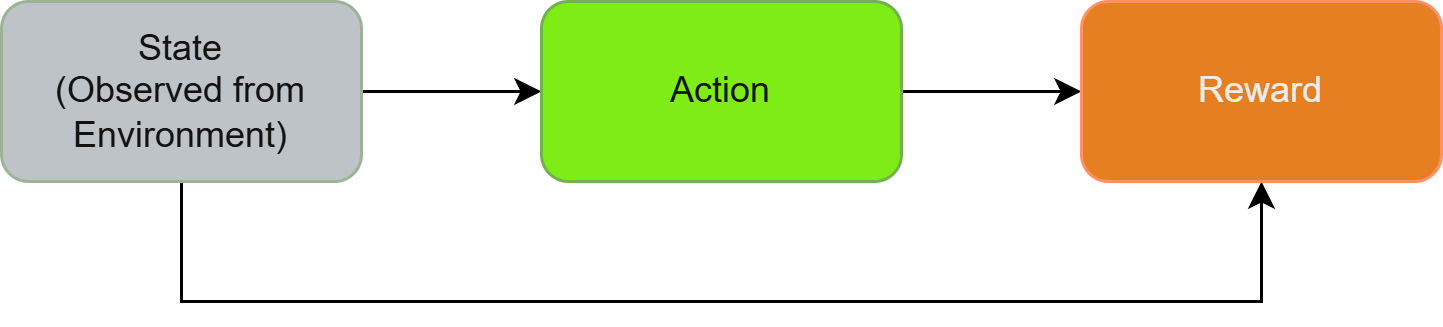
\includegraphics[width=0.49\columnwidth]{images/Networks/contextual_bandit.png}\hfill
  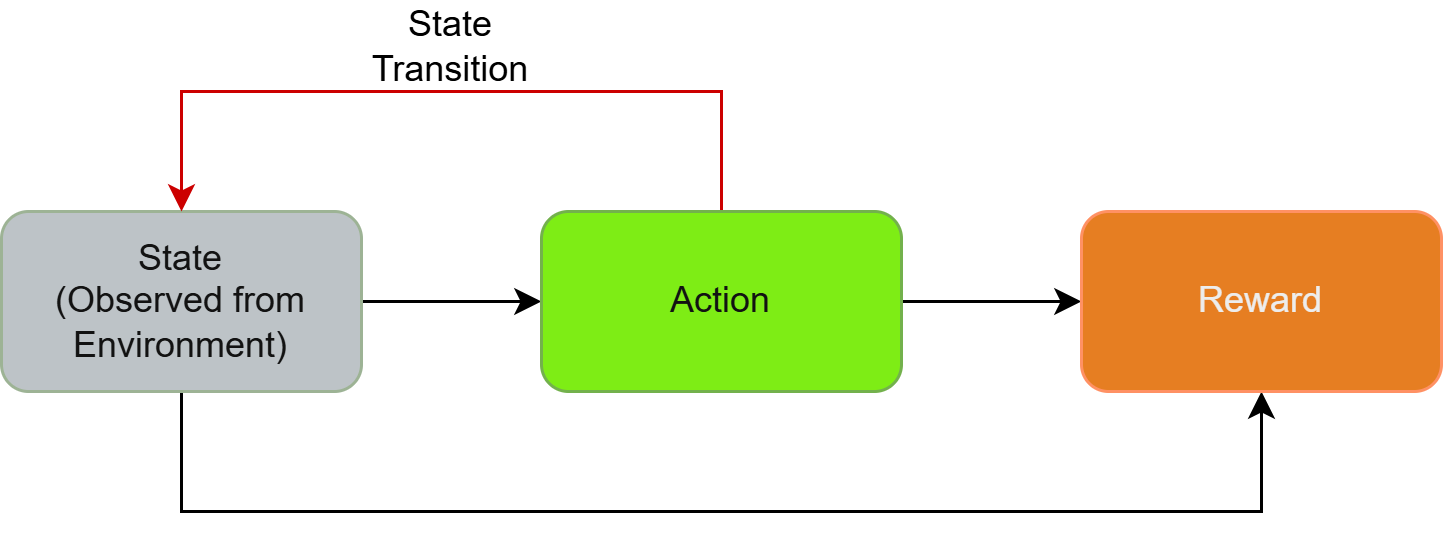
\includegraphics[width=0.49\columnwidth]{images/Networks/full_rl.png}
  \caption{Contextual bandit (left) and full RL (right) interaction loops.}
  \label{fig:rl_diagrams}
\end{figure}

\subsection{Simulated Environment}
\label{sec:env}
\textbf{Traffic.} A training episode samples 50--250 humans and 0--1000 bots, drawing each simulated user's mouse data from a recording in the RL block and each bot's capability $B_s$ uniformly from $\{0,\dots,9\}$. Because human and bot counts vary independently, the number of active users is not a proxy for the bot count (R1.5).

\textbf{Deterministic world (original submission).} A bot is stopped iff $T>B_s$, and humans always pass. It is the $\alpha\to\infty$ limit of the model below and is kept for comparison.

\textbf{Stochastic (``grounded'') world (R1.1).} A bot passes level $T$ with an item-response probability $\sigma(\alpha(B_s+0.5-T))$, $\alpha=1.5$, so strong bots sometimes solve hard challenges and weak bots sometimes solve easy ones. Human pass rates and solve times per level are taken from Bursztein et al.\ \cite{bursztein_humans_2010} and Searles et al.\ \cite{captcha_study_2023} (Table~\ref{tab:params}); a human who fails is lost. After a pass a human may leave with probability $1-e^{-s_T/45\text{\,s}}$. This last term is an \emph{assumption}: we found no study measuring abandonment after a successful solve.

\textbf{Abandonment-at-presentation world (v2, sensitivity).} Replacing that assumption, a human may abandon when a visible challenge is shown (and again before a retry), never after passing, with per-type rates from Searles et al.\ \cite{captcha_study_2023} (2.6--9.2\% for levels 3--9, scaled by their in-context/pooled ratio of 1.34) and a position multiplier that front-loads abandonment ($\times3.25$ for the first challenge, $\times0.55$ from the fourth). An abandoning human is charged $R_{\text{FP}}$, consistent with the metrics, and level 10 blocks everyone. Used only in the pilot of Section~\ref{sec:drift}.

\begin{table}[!t]
\caption{Parameters and Their Sources (R2.4). Lit.\,= Published Study; Search = Chosen by Grouped CV on the RL Block; Assum.\,= Modelling Choice}
\label{tab:params}
\centering
\footnotesize
\setlength{\tabcolsep}{2.5pt}
\begin{tabular}{p{0.55\columnwidth}p{0.18\columnwidth}p{0.17\columnwidth}}
\toprule
\textbf{Parameter} & \textbf{Value} & \textbf{Source} \\
\midrule
\multicolumn{3}{l}{\emph{Environment}} \\
Human pass rate, median s, levels 3--8 & .98/3.7 \dots .70/13 & Lit.\ \cite{bursztein_humans_2010,captcha_study_2023} \\
Level 9 (game) / 10 & .62/25\,s / block & Lit.\ \cite{captcha_study_2023}/Assum. \\
Bot solve slope $\alpha$; $B_s$ & 1.5; $\mathcal U\{0..9\}$ & Assum.\ (sweep 0.5--$\infty$) \\
Leave after pass, $\tau$ & 45\,s & Assum.\ (sweep 22--80) \\
Abandon at presentation (v2) & 2.6--9.2\% & Lit.\ \cite{captcha_study_2023} \\
\midrule
\multicolumn{3}{l}{\emph{Reward}} \\
$R_{\max}$, $R_{\text{leak}}$, $R_{\text{FP}}$ & 50, $-150$, $-100$ & Assum.\ (9-setting sweep) \\
$c_o$, $c_u$, $c_f$ & 2.5, 5, 2/s & Assum.\ (sweep) \\
\midrule
\multicolumn{3}{l}{\emph{Learners}} \\
DQN/PPO body & 128--64 ReLU & Search (6 / 5 bodies) \\
LinUCB / TS embedding & 64--32 / 128--64--64 & Search \\
TS posterior & MoG (2--3 comp.) & Search \\
Episodes; steps/episode & 200; $\le$12 per user & Assum. \\
DQN: $\gamma$, lr, $\epsilon$ decay, target sync & .95, $5\!\times\!10^{-4}$, .9995, 200 & Standard \cite{mnih_dqn_2015} \\
PPO: clip, GAE $\lambda$, epochs, lr & .2, .95, 10, $3\!\times\!10^{-4}$ & Standard \cite{schulman_ppo_2017} \\
LinUCB $\alpha$, ridge $\lambda$ & 1, 1 & Standard \cite{li_linucb_2010} \\
Seeds & 5 train $\times$ 50 eval & --- \\
\bottomrule
\end{tabular}
\end{table}

\subsection{Evaluation Protocol and Metrics}
Each trained policy is evaluated on traffic built from the evaluation block, with 100 humans and $\{20,100,200,500,1000\}$ bots, 50 evaluation seeds per volume, for each of 5 training seeds. Let $S_H$ and $S_B$ be the fractions of humans and bots that complete their session. We report the \textbf{Discrimination Index} $\text{DI}=100(S_H-S_B)$, the \textbf{Balanced Orchestration Score} $\text{BOS}=2S_HK_B/(S_H+K_B)$ with $K_B=1-S_B$ (the F1-style harmonic mean \cite{fscore_2023}), and the scale-invariant $\text{SI-F1}$, the F1 of $S_H$ with normalised precision $S_H/(S_H+S_B)$, plus mean friction in seconds. \emph{Zero-bot traffic is excluded} from every metric and average (R1.4): $S_B$ is undefined without bots, and the original table filled it with conventions that were not stated. Uncertainty is reported \emph{across training seeds} (each seed averaged over volumes and evaluation seeds), as a 95\% $t$-interval; comparisons use Welch's test with Holm correction \cite{holm_1979}. We use ``significant'' only for such tests.

\section{RESULTS}
\label{sec:results}

\subsection{Humanity Scorer}
\textbf{Original model.} On the original temporal hold-out (283 test windows from a later campaign) the original two-layer model reached 90.46\% accuracy, 93.67\% recall and ROC-AUC 0.951 (Table~\ref{tab:confusion}).

\begin{table}[!t]
\caption{Confusion Matrix of the Original Scorer on Its Test Set}
\label{tab:confusion}
\centering
\footnotesize
\begin{tabular}{lcc}
\toprule
 & \textbf{Predicted human} & \textbf{Predicted bot} \\
\midrule
Actual human & 163 & 11 \\
Actual bot & 16 & 93 \\
\bottomrule
\end{tabular}
\end{table}

\textbf{Revised model.} The five cross-fitted scorers used for RL training reach validation AUC 0.950--0.986 and held-out AUC 0.920--0.992. On a pool of unseen sessions, the selected architecture has window AUC 0.954 and session AUC 0.971; temperature scaling reduces the expected calibration error from 0.064 to 0.046, with Brier score 0.065 (R1.7). Leave-one-campaign-out (unseen participant sitting and hardware) lowers session AUC to 0.890, which is the more honest estimate for new users. Fallible bots are the hardest family (AUC 0.918 against humans), human-like bots the easiest (0.991).

\textbf{External data (R1.9).} The original submission reported near-perfect fine-tuned results on the web bot detection dataset of Iliou et al.\ \cite{iliou_2021} and 95.18\% on Balabit \cite{balabit_2016}. On re-examination these numbers do not support a bot-detection claim and we withdraw them: Balabit contains only human users, so its accuracy measured only how many human windows were not flagged, and the web-bot runs split \emph{windows} at random (windows of one session fell on both sides) and used the test set for early stopping. In this revision external data are used only as \emph{unseen populations}, with a session-level split for the web-bot data (advanced bots and humans) and a user-level split for Balabit (5 users for injection, 5 held out). Without fine-tuning the scorer does not transfer: advanced web bots receive a mean $P(\text{bot})$ of only 0.30, and Balabit humans are ranked as more bot-like than those bots (AUC 0.13). This motivates the drift study of Section~\ref{sec:drift}.

\subsection{Main Comparison on Held-Out Recordings}
Table~\ref{tab:headline} replaces Table~4 of the original submission. The original table had two problems: the RL policies were trained and evaluated on the scorer's own test recordings, and its ``$\pm$'' measured variation across bot volumes rather than across training runs. Here every number comes from the held-out evaluation block, and intervals are across 5 training seeds.

\begin{table*}[!t]
\caption{Held-Out Evaluation (Deterministic World, Fold 2). Mean over Bot Volumes 20--1000 (100 Humans) and 50 Evaluation Seeds; Varying Traffic: Humans 64--239 and Bots 3--717 Drawn per Run; $\pm$ Is the 95\% CI over 5 Training Seeds; Static Policies Are Deterministic Given the Scorer}
\label{tab:headline}
\centering
\footnotesize
\resizebox{\textwidth}{!}{\begin{tabular}{lcccccccccccc}
\toprule
 & \multicolumn{5}{c}{\textbf{DI by bot volume}} & & & & & & \\
\cmidrule(lr){2-6}
\textbf{Policy} & 20 & 100 & 200 & 500 & 1000 & \textbf{DI} & \textbf{Worst seed} & \textbf{DI, varying traffic} & \textbf{BOS} & \textbf{SI-F1} & \textbf{Humans kept} & \textbf{Friction (s)} \\
\midrule
DQN & 100.0 & 100.0 & 100.0 & 99.3 & 95.1 & \textbf{98.9} $\pm$ 0.4 & 98.6 & \textbf{99.7} $\pm$ 0.1 & 0.994 & 0.994 & 0.989 & 7.0 \\
Thompson Sampling (MoG3) & 84.7 & 90.7 & 95.0 & 92.0 & 92.3 & 90.9 $\pm$ 12.4 & 73.4 & 88.9 $\pm$ 17.6 & 0.953 & 0.954 & 0.945 & 1.7 \\
LinUCB & 55.4 & 53.8 & 55.1 & 51.4 & 42.0 & 51.5 $\pm$ 36.5 & 13.1 & 49.6 $\pm$ 36.1 & 0.641 & 0.641 & 0.549 & 33.0 \\
Static Multi-Threshold & 80.0 & 78.6 & 78.8 & 78.2 & 78.0 & 78.7 & --- & 78.1 & 0.893 & 0.893 & 0.887 & 9.4 \\
Static Single-Threshold & 77.7 & 77.7 & 77.7 & 77.7 & 77.7 & 77.7 & --- & 77.6 & 0.874 & 0.874 & 0.777 & 6.7 \\
DQN without Humanity Score & 24.8 & 24.1 & 20.2 & 30.5 & 18.3 & 23.6 $\pm$ 10.8 & 13.9 & 21.5 $\pm$ 11.1 & 0.384 & 0.665 & 0.880 & 29.5 \\
\bottomrule
\end{tabular}}
\end{table*}

DQN improves on the best static policy by about 20 DI at every seed (worst seed 98.6 vs 78.7) and keeps all humans up to 200 bots, 95\% at 1000. Removing the Humanity Score from the state costs 75 DI: without it the agent cannot tell users apart and lets 64\% of bots through. Thompson Sampling has the least friction (1.7\,s) but is seed-sensitive (worst seed 73.4), and LinUCB is unstable (13--93). When the numbers of humans (64--239) and bots (3--717) are both varied, drawn independently for each run, the results barely change (DQN 99.7, best static 78.1; Table~\ref{tab:headline}), so the comparison does not depend on a fixed human population. The two counts are drawn per run rather than crossed in a full factorial grid. Two caveats bound these numbers. First, the evaluation block is small (14 human and 36 bot recordings) and the scorer separates it almost perfectly, so DQN is near a ceiling; on the validation folds used for architecture search the same DQN scores 83.6 $\pm$ 0.8 (SE). Second, leakage of training recordings into evaluation would inflate scores: in a role-reversal test (two agents, each evaluated on the recordings it trained on and on those it did not), DQN scores 4.5 DI higher on seen recordings (SE 2.1, 10 splits), while the policies that do not train show a gap of exactly zero. The ranking is unchanged on unseen recordings (DQN 78.2 vs 66.5 for the best static).

\textbf{Population confound (R1.5).} Freezing the active-user feature at any constant from 25 to 800 changes human survival by at most 4.4 points and bot survival by at most 1.8, so security outcomes do not depend on reading the attack size from the population. The \emph{share of users challenged} does depend on it (0.305 unfrozen; 0.204--0.357 frozen), so this feature mainly controls how cautious the policy is.

\subsection{Stochastic Challenge Outcomes}
Table~\ref{tab:e8} repeats the comparison in the grounded world, where challenges are passed probabilistically and humans can fail or leave. Policies retrained in this world are compared with the deterministic-world DQN transferred without retraining.

\begin{table}[!t]
\caption{Grounded Stochastic World ($\alpha=1.5$), Mean over 5 Training Seeds}
\label{tab:e8}
\centering
\footnotesize
\setlength{\tabcolsep}{3pt}
\begin{tabular}{lccccc}
\toprule
\textbf{Policy} & \textbf{DI} & \textbf{Humans} & \textbf{Bots} & \textbf{Aband.} & \textbf{Fric.\,(s)} \\
\midrule
Thompson Sampling (MoG3) & \textbf{91.5} & 0.956 & 0.041 & 0.032 & 2.6 \\
DQN (retrained) & 88.6 & 0.886 & 0.000 & 0.106 & 5.8 \\
DQN (deterministic-trained) & 86.4 & 0.864 & 0.000 & 0.134 & 6.6 \\
Static Single-Threshold & 82.6 & 0.826 & 0.000 & 0.116 & 11.5 \\
Static Multi-Threshold & 80.6 & 0.813 & 0.007 & 0.164 & 9.4 \\
LinUCB & 24.3 & 0.272 & 0.029 & 0.593 & 40.8 \\
DQN without Humanity Score & 7.5 & 0.512 & 0.437 & 0.443 & 24.9 \\
\bottomrule
\end{tabular}
\end{table}

With stochastic outcomes the advantage of DQN over Thompson Sampling disappears: Thompson Sampling has the highest DI at every bot-solve slope tested ($\alpha$ from 0.5 to 12: 90.3--92.2 vs 86.1--86.9 for DQN), mainly because it challenges less and loses fewer humans to abandonment (3.2\% vs 10.6\%). Learned policies still beat static thresholds. The retrained DQN's mean includes one collapsed seed (49.8), which is why its seed SD is 21.7.

\textbf{Reward and abandonment sensitivity (R1.3).} Retraining DQN under nine reward settings (leak penalty, friction form and scale, over- and under-kill coefficients; 5 seeds each) gives a policy that beats every static baseline on the seed mean in all nine; 3 of the 45 runs collapsed. Under the shortest leave-after-pass constant ($\tau=22$\,s) the fixed policies rank DQN 91.7, Static Single 81.4, Thompson Sampling 75.9, Static Multi 64.8, LinUCB 1.8.

\subsection{Rewards a Deployment Could Compute}
\label{sec:deploy}
A deployed controller sees only observable outcomes: a session that failed a challenge and ended may be a blocked bot or a lost human; one that passed may be a satisfied human or a leaked bot. In our simulation 47.5\% of ``passed and continued'' events are bots and 11.6\% of ``failed and ended'' events are humans. We trained DQN with 12 rewards computed from such outcomes (different penalties, potential-based shaping, a learned reward model, delayed abuse labels): \emph{all 12 converged to never challenging anyone} (DI $\approx0$). Two scorer-based alternatives work in the stationary setting: a \emph{score-only} reward that replaces the class label with the score (DI 85.3, seed SD 8.3), and a \emph{posterior} reward that weights the oracle reward by the posterior class probability, using an EM estimate of the current bot share (DI 92.8, SD 5.9; oracle 88.6). Neither difference from the oracle is significant ($p=0.70$ and $p=0.15$ before correction). The posterior reward uses the simulator's own outcome model and is therefore an upper bound for this idea, and both rewards rely on the scorer being right, which the next section tests.

\subsection{Calibration Drift: Offline vs Online Training}
\label{sec:drift}
We simulate a scorer whose calibration degrades. In the \emph{bots-look-human} direction a fraction $\rho$ of evaluation bots is replaced by advanced web bots from an external dataset \cite{iliou_2021}, which the scorer rates as human-like; in the \emph{humans-look-bot-like} direction a fraction $\rho$ of humans is replaced by Balabit users \cite{balabit_2016}. As $\rho$ goes from 0 to 1 the calibration error of the shifted class grows from 0.07 to 0.61 (bots) and from 0.13 to 0.45 (humans), while session-level AUC stays $\ge0.99$, i.e., the ranking of sessions barely changes but the score's probabilities become wrong. We compare (a) policies trained offline and evaluated frozen, and (b) DQN and PPO trained online for 300 episodes, with the shift injected from episode 100, against the same protocol without the shift (control). The scorer is a cross-fitted seed chosen because it ranks the external bots best; this choice was made after inspecting the external data.

\begin{figure*}[!t]
  \centering
  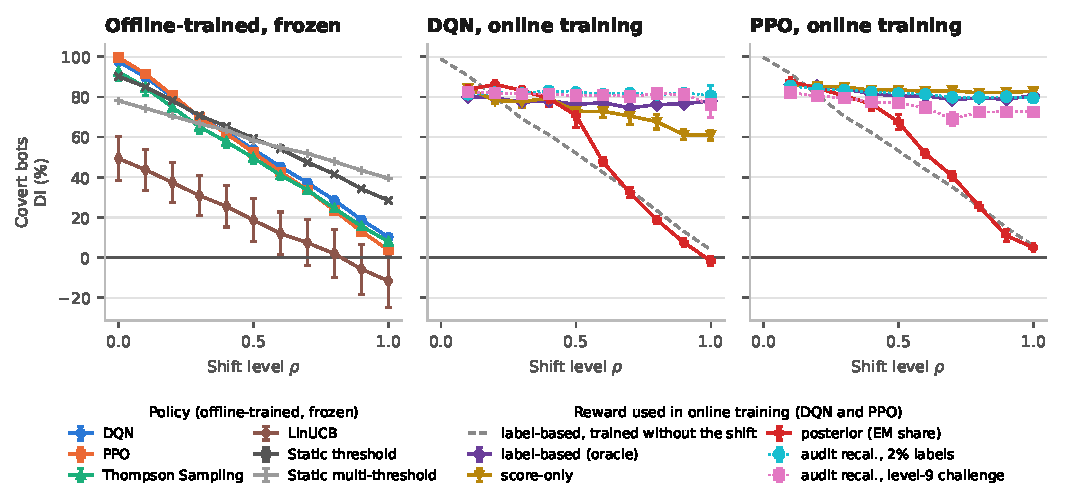
\includegraphics[width=0.92\textwidth]{images/drift.pdf}
  \caption{DI on the held-out block as the scorer's calibration degrades (grounded world, mean $\pm$ SE over 5 training seeds). Left: offline-trained policies, frozen. Middle/right: online training through the shift with three rewards; dashed: oracle reward trained without the shift. Online points start at $\rho=0.1$.}
  \label{fig:drift}
\end{figure*}

\textbf{Offline-trained, frozen} (Fig.~\ref{fig:drift}, left). All score-using policies degrade as calibration error grows; DQN without the score stays flat at about 16, as expected for a negative control. When bots look human, the RL policies fall \emph{further} than static thresholds (at $\rho=1$: DI 10.2 DQN, 3.8 PPO vs 28.4 and 39.5 static), because they rely on the score more. When humans look bot-like the order reverses (57.9 DQN, 56.4 PPO vs 22.5 and 26.3 static).

\textbf{Online training} (middle and right). Averaged over $\rho$ and tested against the no-shift control (Holm over 24 contrasts), the oracle reward recovers the bot shift significantly ($+30.5$ DQN, $+33.2$ PPO DI; $p_{\text{holm}}<10^{-6}$) and the score-only reward also does ($+27.6$, $+27.5$; $p_{\text{holm}}\le0.003$). The score-only reward cannot recover the human shift (PPO $-8.7$, $p_{\text{holm}}=0.002$). No posterior-family reward gains significantly in either direction, and at $\rho=1$ with covert bots online training with the posterior reward lets essentially every bot through (DI $\approx0$), \emph{below} its own no-shift control: the reward inherits the scorer's error and teaches it to the policy.

\textbf{Pilot in the v2 world.} To check that these conclusions do not depend on the leave-after-pass assumption, we repeated the study in the abandonment-at-presentation world with a 7-feature state (adding the highest level solved and the number of steps passed). This pilot uses one seed and the validation block, so it is indicative only (Table~\ref{tab:pilot}). The pattern is the same: frozen policies collapse under covert bots, oracle online training recovers both directions, and the posterior reward collapses.

\begin{table}[!t]
\caption{v2-World Pilot at Full Shift ($\rho=1$): DI, One Seed, Validation Block. At $\rho=0$ Offline DI Is 100.0 (DQN), 99.8 (PPO), 84.5 (TS)}
\label{tab:pilot}
\centering
\footnotesize
\setlength{\tabcolsep}{3pt}
\begin{tabular}{lcccccc}
\toprule
 & \multicolumn{3}{c}{\textbf{Bots look human}} & \multicolumn{3}{c}{\textbf{Humans look bot-like}} \\
\cmidrule(lr){2-4}\cmidrule(lr){5-7}
\textbf{Training} & DQN & PPO & TS & DQN & PPO & TS \\
\midrule
Offline, frozen & 8.9 & 7.6 & $-7.3$ & 46.2 & 48.7 & 50.5 \\
Online, oracle & 69.6 & 54.3 & 61.9 & 61.4 & 70.4 & 75.0 \\
Online, score-only & 62.0 & 39.9 & 22.5 & 18.0 & 18.0 & 17.9 \\
Online, posterior & 0.3 & 5.0 & 3.5 & 17.2 & 13.3 & 16.7 \\
\bottomrule
\end{tabular}
\end{table}

\section{DISCUSSION AND LIMITATIONS}
\textbf{What the evidence supports.} With a well-calibrated behavioural score, a learned controller separates humans from bots better than static thresholds on held-out recordings, the score is the component that matters most, and the advantage holds when challenge outcomes are stochastic, although the best learner then changes from DQN to Thompson Sampling.

\textbf{What it does not.} (1) \emph{Deployment reward}: the policies need the true class during training. Rewards from observable outcomes fail, and scorer-based rewards are only as good as the scorer; a deployment would need periodic labelled data (e.g., confirmed abuse or manual review) for oracle-style updates and a monitor of the scorer's calibration. (2) \emph{Usability is modelled, not measured}: pass rates, times and abandonment come from published studies of other populations, and no participant interacted with the 11 levels. (3) \emph{Data}: 3 human participants and 4 bot generators; the evaluation block is small and near ceiling. (4) \emph{Simulator}: no real CAPTCHA provider, no request-rate, CPU or latency model (hence no server-resource DoS claim), and no adaptive or VLM-based attacker, although the drift study shows what happens when unseen bots arrive. (5) \emph{Post-hoc choice}: the drift-study scorer seed was chosen after seeing the external data.

\textbf{Future work.} A multi-seed run of the v2 world with the extended state and a label-free reward with a fixed bot-share prior is in progress. Beyond it: a user study of the challenge ladder, integration with real CAPTCHA providers, a queueing model for server load, and attackers that adapt to the learned policy.

\section{CONCLUSION}
We framed CAPTCHA orchestration as learning a mapping from a calibrated behavioural score and session context to an 11-level challenge ladder, and evaluated it in a simulator grounded in published CAPTCHA user studies with a leakage-controlled data protocol. On held-out recordings DQN reaches 98.9 DI ($\pm$0.4 over seeds) against 78.7 for the best static policy, and without the score it drops to 23.6; with stochastic challenge outcomes Thompson Sampling performs best. The same experiments show where the approach stops: no reward computed from observable outcomes alone trained a working policy, and policies trained or adapted with scorer-derived rewards inherit the scorer's miscalibration. A practical system therefore needs a calibrated scorer, a source of occasional ground-truth labels, and calibration monitoring; with those, RL is a viable replacement for hand-tuned score thresholds.

\section*{ACKNOWLEDGMENT}
AI tools were used for language editing and formatting. The authors thank the participants who provided mouse-movement data.

\begin{thebibliography}{10}
\bibitem{imperva2025} Imperva, ``2025 Imperva Bad Bot Report,'' Thales Group, 2025.
\bibitem{mazilu2022} M.~C.~Mazilu, ``Web scraping and ethics in automated data collection,'' in \emph{Smart Innovation, Systems and Technologies}, vol.~276. Springer, 2022.
\bibitem{ferrara2016} E.~Ferrara, O.~Varol, C.~Davis, F.~Menczer, and A.~Flammini, ``The rise of social bots,'' \emph{Commun. ACM}, vol.~59, no.~7, pp.~96--104, 2016.
\bibitem{ba2021} M.~H.~N.~Ba, J.~Bennet, M.~Gallagher, and S.~Bhunia, ``A case study of credential stuffing attack: Canva data breach,'' in \emph{Proc. Int. Conf. Comput. Sci. Comput. Intell. (CSCI)}, 2021.
\bibitem{von_2003} L.~von~Ahn, M.~Blum, N.~J.~Hopper, and J.~Langford, ``CAPTCHA: Using hard AI problems for security,'' in \emph{Advances in Cryptology -- EUROCRYPT 2003}, pp.~294--311.
\bibitem{guerar2021} M.~Guerar, L.~Verderame, M.~Migliardi, F.~Palmieri, and A.~Merlo, ``Gotta CAPTCHA 'em all: A survey of 20 years of the human-or-computer dilemma,'' \emph{ACM Comput. Surv.}, vol.~54, no.~9, Art.~192, 2021.
\bibitem{bursztein_humans_2010} E.~Bursztein, S.~Bethard, C.~Fabry, J.~C.~Mitchell, and D.~Jurafsky, ``How good are humans at solving CAPTCHAs? A large scale evaluation,'' in \emph{Proc. IEEE Symp. Security and Privacy}, 2010, pp.~399--413, doi: 10.1109/SP.2010.31.
\bibitem{captcha_study_2023} A.~Searles, Y.~Nakatsuka, E.~Ozturk, A.~Paverd, G.~Tsudik, and A.~Enkoji, ``An empirical study \& evaluation of modern CAPTCHAs,'' in \emph{Proc. 32nd USENIX Security Symp.}, 2023, pp.~3081--3097.
\bibitem{qi2026} M.~Qi \emph{et al.}, ``VIPER Strike: Defeating visual reasoning CAPTCHAs via structured vision-language inference,'' arXiv:2601.06461, 2026.
\bibitem{wu2025mca_bench} Z.~Wu \emph{et al.}, ``MCA-Bench: A multimodal benchmark for evaluating CAPTCHA robustness against VLM-based attacks,'' arXiv:2506.05982, 2025.
\bibitem{plesner2024yolo} A.~Plesner, T.~Vontobel, and R.~Wattenhofer, ``Breaking reCAPTCHAv2,'' in \emph{Proc. IEEE COMPSAC}, 2024.
\bibitem{reCAPTCHA} Google reCAPTCHA. [Online]. Available: \url{https://www.google.com/recaptcha/about}
\bibitem{sepczuk_2018} M.~Sepczuk and Z.~Kotulski, ``A new risk-based authentication management model oriented on user's experience,'' \emph{Comput. Secur.}, vol.~73, pp.~17--33, 2018.
\bibitem{sethi_2018} T.~S.~Sethi, M.~Kantardzic, L.~Lyu, and J.~Chen, ``A dynamic-adversarial mining approach to the security of machine learning,'' \emph{WIREs Data Mining Knowl. Discov.}, vol.~8, 2018.
\bibitem{sivakorn_recaptcha_2016} S.~Sivakorn, J.~Polakis, and A.~D.~Keromytis, ``I'm not a human: Breaking the Google reCAPTCHA,'' in \emph{Black Hat Asia}, 2016.
\bibitem{yousef_2023} W.~A.~Yousef, I.~Traor\'e, and W.~Briguglio, ``Classifier calibration: With application to threat scores in cybersecurity,'' \emph{IEEE Trans. Dependable Secure Comput.}, vol.~20, no.~3, pp.~1994--2010, 2023.
\bibitem{cloudArmour} Google Cloud Armor. [Online]. Available: \url{https://cloud.google.com/security/products/armor}
\bibitem{umar_2022} M.~Umar and S.~Ayyub, ``A review on evolution of various CAPTCHA in the field of web security,'' \emph{IJRASET}, 2022.
\bibitem{yan2008captcha} J.~Yan and A.~S.~El~Ahmad, ``Usability of CAPTCHAs or usability issues in CAPTCHA design,'' in \emph{Proc. SOUPS}, 2008.
\bibitem{bursztein2014new} E.~Bursztein, J.~Aigrain, A.~Moscicki, and J.~C.~Mitchell, ``The end is nigh: Generic solving of text-based CAPTCHAs,'' in \emph{Proc. USENIX WOOT}, 2014.
\bibitem{akrout2019} I.~Akrout, A.~Feriani, and M.~Akrout, ``Hacking Google reCAPTCHA v3 using reinforcement learning,'' arXiv:1903.01003, 2019.
\bibitem{clip_2021} A.~Radford \emph{et al.}, ``Learning transferable visual models from natural language supervision,'' in \emph{Proc. ICML}, PMLR vol.~139, pp.~8748--8763, 2021.
\bibitem{khan_2023} S.~Khan, C.~Devlen, M.~Manno, and D.~Hou, ``Mouse dynamics behavioral biometrics: A survey,'' \emph{ACM Comput. Surv.}, vol.~56, no.~6, pp.~1--33, 2024, doi: 10.1145/3640311.
\bibitem{shen_2013} C.~Shen, Z.~Cai, X.~Guan, and J.~Wang, ``Mouse dynamics for continuous user authentication: An experimental analysis,'' in \emph{Proc. NSS}, Springer, 2013, pp.~250--261.
\bibitem{antal_2019} M.~Antal and E.~Egyed-Zsigmond, ``Intrusion detection using mouse dynamics,'' \emph{IET Biometrics}, vol.~8, no.~5, pp.~285--294, 2019.
\bibitem{fittslaw2019} M.~Takeda, T.~Sato, H.~Saito, H.~Iwasaki, I.~Nambu, and Y.~Wada, ``Explanation of Fitts' law in reaching movement based on human arm dynamics,'' \emph{Sci. Rep.}, vol.~9, Art.~19804, 2019.
\bibitem{bezier2025} S.~Adarsh, P.~V.~V.~Sankaranarayanan, and P.~A.~Suresh, ``Emulating human-like mouse movement using B\'ezier curves and behavioural models for advanced web automation,'' \emph{IJIRT}, vol.~12, no.~1, 2025.
\bibitem{bezier_bots_2022} A.~Acien, A.~Morales, J.~Fierrez, and R.~Vera-Rodriguez, ``BeCAPTCHA-Mouse: Synthetic mouse trajectories and improved bot detection,'' \emph{Pattern Recognit.}, vol.~127, 2022.
\bibitem{antal_2021_sapi} M.~Antal, K.~Buza, and N.~Fejer, ``SapiAgent: A bot based on deep learning to generate human-like mouse trajectories,'' \emph{IEEE Access}, vol.~9, 2021.
\bibitem{iliou_2021} C.~Iliou, T.~Kostoulas, T.~Tsikrika, V.~Katos, S.~Vrochidis, and I.~Kompatsiaris, ``Detection of advanced web bots by combining web logs with mouse behavioural biometrics,'' \emph{Digit. Threats: Res. Pract.}, vol.~2, no.~3, Art.~24, 2021, doi: 10.1145/3447815.
\bibitem{acien_2021} A.~Acien, A.~Morales, J.~Fierrez, R.~Vera-Rodriguez, and O.~Delgado-Mohatar, ``BeCAPTCHA: Behavioral bot detection using touchscreen and mobile sensors benchmarked on HuMIdb,'' \emph{Eng. Appl. Artif. Intell.}, vol.~98, 2021.
\bibitem{hochreiter_lstm_1997} S.~Hochreiter and J.~Schmidhuber, ``Long short-term memory,'' \emph{Neural Comput.}, vol.~9, no.~8, pp.~1735--1780, 1997, doi: 10.1162/neco.1997.9.8.1735.
\bibitem{wei2021deeplearning} D.~Wei \emph{et al.}, ``Predicting mouse click position using long short-term memory model trained by joint loss function,'' in \emph{Proc. CHI EA}, 2021.
\bibitem{aura_captcha_2025} R.~Sahay \emph{et al.}, ``Aura-CAPTCHA: A reinforcement learning and GAN-enhanced multi-modal CAPTCHA system,'' arXiv:2508.14976, 2025.
\bibitem{li_linucb_2010} L.~Li, W.~Chu, J.~Langford, and R.~E.~Schapire, ``A contextual-bandit approach to personalized news article recommendation,'' in \emph{Proc. 19th Int. Conf. World Wide Web}, 2010, pp.~661--670, doi: 10.1145/1772690.1772758.
\bibitem{russo_ts_2018} D.~J.~Russo, B.~Van~Roy, A.~Kazerouni, I.~Osband, and Z.~Wen, ``A tutorial on Thompson sampling,'' \emph{Found. Trends Mach. Learn.}, vol.~11, no.~1, pp.~1--96, 2018, doi: 10.1561/2200000070.
\bibitem{mnih_dqn_2015} V.~Mnih \emph{et al.}, ``Human-level control through deep reinforcement learning,'' \emph{Nature}, vol.~518, no.~7540, pp.~529--533, 2015, doi: 10.1038/nature14236.
\bibitem{schulman_ppo_2017} J.~Schulman, F.~Wolski, P.~Dhariwal, A.~Radford, and O.~Klimov, ``Proximal policy optimization algorithms,'' arXiv:1707.06347, 2017.
\bibitem{sutton2018reinforcement} R.~S.~Sutton and A.~G.~Barto, \emph{Reinforcement Learning: An Introduction}, 2nd~ed. MIT Press, 2018.
\bibitem{cui_2025} Y.~Cui, X.~Han, J.~Chen, X.~Zhang, J.~Yang, and X.~Zhang, ``FraudGNN-RL: A graph neural network with reinforcement learning for adaptive financial fraud detection,'' \emph{IEEE Open J. Comput. Soc.}, 2025.
\bibitem{huang_2018} C.~Huang, Y.~Wu, Y.~Zuo, K.~Pei, and G.~Min, ``Towards experienced anomaly detector through reinforcement learning,'' in \emph{Proc. AAAI}, 2018.
\bibitem{mvula_2023} P.~K.~Mvula, P.~Branco, G.-V.~Jourdan, and H.~L.~Viktor, ``A systematic literature review of cyber-security data repositories and performance assessment metrics for semi-supervised learning,'' \emph{Discover Data}, 2023.
\bibitem{guo_calibration_2017} C.~Guo, G.~Pleiss, Y.~Sun, and K.~Q.~Weinberger, ``On calibration of modern neural networks,'' in \emph{Proc. ICML}, 2017, pp.~1321--1330.
\bibitem{fscore_2023} P.~Christen, D.~J.~Hand, and N.~Kirielle, ``A review of the F-measure: Its history, properties, criticism, and alternatives,'' \emph{ACM Comput. Surv.}, vol.~56, no.~3, Art.~73, 2023.
\bibitem{holm_1979} S.~Holm, ``A simple sequentially rejective multiple test procedure,'' \emph{Scand. J. Statist.}, vol.~6, no.~2, pp.~65--70, 1979.
\bibitem{balabit_2016} \'A.~F\"ul\"op, L.~Kov\'acs, T.~Kurics, and E.~Windhager-Pokol, Balabit Mouse Dynamics Challenge data set, 2016. [Online]. Available: \url{https://github.com/balabit/Mouse-Dynamics-Challenge}
\end{thebibliography}

\end{document}
